\chapter{Revisión del estado de la técnica}

Antes de poder aventurarnos el desarrollo de una herramienta para la
orquestación de tareas de tiempo real usando contenedores, es necesario
estudiar y comprender los fundamentos y peculiaridades de diversos campos como
son los sistemas de tiempo real, la planificación de procesos, la computación en
la nube o las tecnologías de virtualización. En este capítulo, se introducen los
conceptos más importantes de estos campos, además de revisar otros trabajos
realizados con el objetivo de comprobar cuál es el estado de la investigación
en dichos temas.

\section{Sistemas empotrados, confiables y de criticalidad mixta}

Los ordenadores y teléfonos inteligentes que usamos a diario nos permiten
realizar multitud de tareas diferentes: desde leer el correo o navegar por
internet hasta editar imágenes y vídeos o realizar videollamadas. Aunque no nos
demos cuenta, interactuamos habitualmente con muchos más sistemas informáticos
además de los ya mencionados. La computación está presente en los coches, los
trenes, los aviones, los satélites espaciales, los televisores o las lavadoras.
Estos sistemas, que reciben el nombre de sistemas empotrados, son diseñados para
llevar a cabo de manera óptima un conjunto de tareas específico, frente al
enfoque generalista de los ordenadores de uso personal. Como se introduce en
\cite{wolf_high-performance_2014}, los sistemas empotrados son comunes en
contextos en los que el rendimiento es primordial, como son las comunicaciones
de red o la compresión/decompresión de audio y vídeo para retransmisiones en
directo. En este libro se exponen diversas aplicaciones de los sistemas
empotrados de alto rendimiento para sistemas ciber-físicos o CPS
(\textit{Cyber-Physical Systems}). Los CPS son, en esencia, sistemas
informáticos que interactúan con procesos físicos, actuando en función de los
cambios en su entorno. Este aspecto hace que el diseño y la implementación de
los CPS difiera considerablemente del resto de sistemas empotrados, ya que hay
que prestar especial atención a las características del entorno en el que se
desplegará el sistema y a los mecanismos de entrada y salida (interacción con el
entorno), además de optimizar el consumo de memoria y procesamiento para cumplir
con las limitaciones del hardware \cite{lee_introduction_2016}.

En algunos casos, estos sistemas son críticos, lo que significa que un fallo en
su funcionamiento supone daños graves a las personas o al medio ambiente. Este
es el caso de los aviones, los trenes o las plantas nucleares, por ejemplo. En
estos sistemas, cobra especial importancia el concepto de confiabilidad, es
decir, garantizar el correcto funcionamiento del sistema en todo momento. En la
figura \ref{fig:01-dependability} se pueden apreciar los atributos que debe
poseer un sistema confiable. A nivel de software, existen arquitecturas y
patrones de diseño orientados a garantizar la tolerancia ante los fallos del
mismo \cite{pullum_software_2001}\cite{randell_system_1975}. Por otra parte, la
replicación de componentes \cite{hutchison_dependable_2006} es una técnica muy
usada tanto para el software como el hardware. Lo que se intenta con la
replicación es asegurar que un cálculo o procesamiento se lleva a cabo de forma
correcta, aunque alguna de las réplicas falle. En \cite{amin_review_2019}, se
realiza una revisión de los sistemas de control tolerantes ante fallos
dividiéndolos en tres tipos: AFTCS (\textit{Active Fault Tolerant Control
  Systems}), PFTCS (\textit{Passive Fault Tolerant Control Systems}) o HFTCS
(\textit{Hybrid Fault Tolerant Control Systems}). Para cada uno de estos tipos,
los autores presentan las principales arquitecturas usadas, los modelos de
análisis matemático usados para su validación y las últimas técnicas usadas para
su diseño. Por otra parte, el estudio realizado en \cite{shan_survey_2019} tiene
como objetivo analizar la aplicación de los estándares de seguridad, protección
y privacidad al diseño y desarrollo de sistemas confiables, llegando los autores
a la conclusión de que cada vez están ganando más popularidad los de protección
y privacidad, aunque los procesos para asegurar estos aspectos son menos maduros
que los relacionados con la seguridad. Además, también se identifica una falta
de acción combinada en estos aspectos, trabajando normalmente por separado en
cada uno de ellos.

\begin{figure}
  \centering
  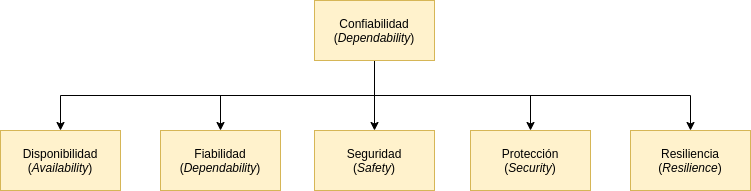
\includegraphics[width=\textwidth]{01-introduction/dependability.png}
  \caption{Principales aspectos de la confiabilidad}
  \label{fig:01-dependability}
\end{figure}

Para muchos sistemas de control, el tiempo es también un aspecto relevante a la
hora de garantizar su correcto funcionamiento. Estos son los llamados sistemas
de tiempo real. En un sistema normal, en el que se obtiene una salida al aplicar
una cierta lógica sobre la entrada, la corrección de dicha salida depende de la
corrección de la lógica aplicada, es decir, del cálculo realizado. No obstante,
cuando hablamos de sistemas de tiempo real, la corrección de la lógica no es
suficiente para determinar que el funcionamiento es correcto, sino que esta
corrección depende también del momento temporal en el que se obtiene
\cite{gambier_real-time_2004}. En otras palabras, si el cálculo es correcto pero
el resultado no llega en el momento en el que se necesita, se considera como un
fallo del sistema. Las tareas que ejecuta un sistema de tiempo real están, por
tanto, sujetas a restricciones temporales. Normalmente, hablamos de un tiempo
límite o \textit{deadline} antes del cuál se debe haber completado la tarea.
Comúnmente, se suelen clasificar las tareas en dos tipos dependiendo de las
consecuencias de incumplir con sus restricciones temporales:

\begin{itemize}
  \item Tareas de tiempo real «blandas»: Se denominan así aquellas tareas en las
        que no completar las mismas antes del límite supone una reducción en la
        calidad del servicio (QoS).
  \item Tareas de tiempo real «duras»: En estas tareas, el no cumplir con las
        restricciones temporales supone un fallo grave del sistema con posibles
        consecuencias catastróficas.
\end{itemize}

Para implementar estos sistemas, se hace uso de herramientas y algoritmos de
planificación de procesos específicos que permiten la ejecución de estos tipos
de tareas cumpliendo con sus restricciones temporales. Esto se explica en más
detalle en la sección \ref{sec:real-time}.

En este trabajo, nos centraremos especialmente en los sistemas de control
aplicados a entornos industriales. Debemos diferenciar entre dos conceptos: PCS
(\textit{Process Control System}), que es el sistema encargado de controlar una
parte concreta de la planta (p. ej., una turbina o un brazo robótico), e ICS
(\textit{Industrial Control System}), que se refiere al control de toda la
planta al completo. Un ICS está compuesto, por tanto, de múltiples PCS que se
encargan de controlar los distintos aspectos del proceso de producción. Estos
PCSs son sistemas empotrados como los que hemos comentado a los que se aplican
también los conceptos de confiabilidad y seguridad. En
\cite{krotofil_industrial_2013} se realiza un estudio del estado del arte en
cuanto a la seguridad de los ICS, concluyendo que, aunque las vulnerabilidades
de muchos de los sistemas actuales son conocidas, la aplicación de parches que
las solucionen son inviables debido a los altos costes asociados a la
recertificación o directamente debido a la incompatibilidad con algunos sistemas
más antiguos. Es necesario, por tanto, incorporar los conceptos de seguridad a
los procesos de diseño desde el primer momento para evitar dar lugar a estas
situaciones.

En 2007, Vestal \cite{vestal_preemptive_2007} publica una primera propuesta para
la planificación de conjuntos de tareas de criticalidad mixta. Este importante
avance es considerado por muchos como el inicio de la investigación en sistemas
de criticalidad mixta o MCS (\textit{Mixed-Criticality Systems}). La idea detrás
de estos sistemas es, como su propio nombre indica, poder ejecutar sobre una
misma plataforma hardware tanto tareas críticas como tareas no críticas o con
niveles de criticalidad menores, asegurando en todo momento que las
restricciones temporales se cumplen, al menos para las tareas más críticas.
Desde entonces, se han planteado muchos modelos para la implementación de estos
sistemas. En \cite{burns_mixed_2015}, Burns realiza una revisión de toda la
investigación realizada en este campo hasta marzo de 2019. Se muestran en esta
revisión algunas arquitecturas propuestas, además de las principales técnicas de
análisis para estos sistemas en plataformas uniprocesador y multiprocesador.
Burns identifica la conciliación entre la separación de los procesos y la
compartición de los recursos como el principal problema de los MCS. En este
aspecto, nuestro trabajo propone el uso de contenedores como medio de ejecución
de los distintos procesos sobre una misma plataforma consiguiendo esa
separación.

No podemos terminar nuestra revisión de los sistemas empotrados sin hablar sobre
el uso del kernel de Linux para su implementación. Como referencia, hemos tomado
dos estudios realizados en 2004 sobre el uso de Linux para sistemas empotrados
\cite{geer_survey_2004}\cite{henkel_munichmit_2004}. En el primero, se destaca
la buena situación de Linux en este campo, suponiendo las soluciones comerciales
basadas en el kernel de Linus Torvalds el 15,5\% del mercado. El segundo estudio
es una encuesta realizada a 268 personas que trabajan en el campo de los
sistemas empotrados, ya sea académicamente o de forma comercial. Lo más
destacable es que la mayoría de los participantes usan Linux en sistemas
empotrados para comunicaciones, dispositivos móviles o control de maquinaria.
Esto último es especialmente alentador para este trabajo, en el que pretendemos
usar Linux como base para la implementación de ICS.

\section{La nube en los sistemas industriales: fog/edge computing para sistemas
  de tiempo real}

Desde su aparición alrededor de 2006, la computación en la nube o \textit{cloud
  computing} ha experimentado un crecimiento abismal, cambiando completamente la
manera en la que las organizaciones gestionan su infraestructura y en la que los
usuarios acceden a servicios. Atendiendo a la definición del NIST
\cite{mell_nist_2011}, se trata de un modelo de prestación de servicios que
ofrece acceso ubicuo, prácticamente ilimitado y bajo demanda a un conjunto de
recursos de computación (p. ej., almacenamiento, tiempo de procesamiento,
comunicaciones), todo ello a través de internet. Sus principales características
son:

\begin{itemize}
  \item Acceso bajo demanda: El consumidor es el que decide qué recursos
        necesita y en qué cantidad, sin necesidad de intervención humana por parte del
        proveedor del servicio.
  \item Consumo a través de internet: El acceso a estos recursos se realiza
        mediante los protocolos ya conocidos y bien establecidos que potencian la web
        (p. ej., HTTP), permitiendo así un acceso ubicuo.
  \item Acceso compartido: Los recursos del proveedor se uniformizan, formando
        una especie de bolsa de recursos que es usada por múltiples consumidores
        (\textit{multi-tenant}). Por ejemplo, aunque desde el punto de vista de un
        usuario pueda parecer que tiene una CPU para él solo, en realidad la CPU
        física es usada por varios usuarios a la vez.
  \item Elasticidad: Dependiendo de la demanda, se pueden asignar o liberar los
        recursos de forma dinámica, consiguiente sistemas más eficientes y capaces de
        dar respuesta a cargas de trabajo más altas.
  \item Servicio medido: El uso de los recursos se monitoriza de forma
        automática, lo que proporciona transparencia tanto para el consumidor como el
        proveedor.
\end{itemize}

A raíz de la propuesta de la computación en la nube, han surgido varios modelos
de prestación de servicios a usuarios. Según el tipo de recurso que ofrecen,
estos modelos se pueden clasificar principalmente en SaaS (\textit{Software as
  a Service}), PaaS (\textit{Platform as a Service}) o IaaS
(\textit{Infrastructure as a Service}). Desde el punto de vista de los usuarios,
estos modelos tienen el beneficio de que permiten pagar solo por lo que
necesitas en cada momento, adaptándose perfectamente a tus necesidades. Además,
estos usuarios ya no se ven limitados por el hardware que poseen. Prácticamente
cualquier ordenador es capaz de conectarse a internet y, de esta forma, acceder
a unos recursos prácticamente ilimitados en la nube. Esto es especialmente
evidente para las empresas, las cuáles ya no necesitan mantener su propia
infraestructura de hardware para soportar su operación diaria, con los enormes
costes y complicaciones que esto supone.

En el campo del control industrial, en el que se centra este trabajo, podríamos
pensar en la nube como una plataforma ideal para procesar las enormes cantidades
de datos que producen las plantas e implementar las técnicas de aprendizaje
automático necesarias para mejorar su autonomía. No obstante, existe un gran
problema: la latencia. En el modelo de la nube, todo el procesamiento está
centralizado en un centro de datos\footnote{Normalmente, existen varios centros
  de datos distribuidos geográficamente, pero a efectos del problema que se
  plantea, se sigue viendo como una «centralización».}, el cuál se encuentra lejos
de la planta donde se recogen los datos. Enviar estos datos a la nube y esperar
una respuesta supone demasiado tiempo como para poder considerar delegar en ella
tareas de control de la operación de la planta. En entornos controlados, donde
el centro de datos se encuentra relativamente cerca de la planta, las pruebas
llevadas a cabo en \cite{hofer_industrial_2019} indican que la latencia puede
ser lo suficientemente predecible para la implementación de ciertos sistemas de
control con requisitos temporales suaves. Sin embargo, se trata de una situación
poco factible, ya que es inviable ubicar un centro de datos cerca de todas las
instalaciones industriales. En \cite{piggin_are_2015}, se analiza si los
ICS están preparados para ser desplazados a la nube, pero centrándose más en el
aspecto de la seguridad de estos sistemas. El autor identifica que, aunque la
nube es una plataforma muy robusta, también son flagrantes las dudas que produce
en cuanto a su seguridad frente a ataques. Por estas razones, no consideramos
que la nube sea un paradigma adecuado para dar respuesta a los nuevos requisitos
de la industria.

Aunque la nube no sea viable, bien es cierto que las ideas de elasticidad y
ubicuidad que plantea son interesantes para el problema en cuestión. Al final
del día, si queremos realizar análisis en tiempo real de los datos que generan
los procesos industriales para tomar decisiones, necesitamos más potencia
computacional de la que ningún dispositivo individual nos puede ofrecer. ¿La
solución? Aprovechar los recursos de computación de todos los dispositivos ya
presentes en las plantas industriales. De acercar estas ideas de la nube a los
dispositivos del borde de la red surgen dos nuevos paradigmas de computación:
\textit{fog} y \textit{edge computing}. En estos paradigmas, se pretende acercar
el procesamiento que se realiza sobre los datos a los propios dispositivos que
generan dichos datos. En el contexto industrial, esto también supone estar más
cerca de los dispositivos que deben actuar en respuesta a este procesamiento,
con lo que se obtendrían tiempos de respuesta mejores que con la nube. La
diferencia entre \textit{fog} y \textit{edge} radica en lo cerca del borde de la
red que ubiquemos el procesamiento de los datos, si bien es cierto que en
algunos escritos se usan los términos \textit{fog} y \textit{edge} de manera
intercambiable \cite{shi_edge_2019}, sin diferencia aparente entre ambos.

\begin{itemize}
  \item En \textit{fog}, se trata de nodos ubicados en la misma red local que
        las fuentes de datos.
  \item En \textit{edge}, los propios dispositivos que generan los datos ya
        realizan un cierto procesamiento de los mismos.
\end{itemize}

En la figura \ref{fig:02-cloud_fog_edge} se puede apreciar como estos dos
paradigmas, junto con la nube, constituyen una arquitectura por capas, donde
cada uno de ellos tiene unas características concretas. Se trata, por tanto, de
modelos complementarios, no exclusivos. En la capa \textit{edge}, donde se
generan los datos, se pueden implementar los mecanismos de control con
restricciones más duras, ya que se tienen unos tiempos de respuesta más rápidos
al actuar directamente en base a los datos generados. En la capa \textit{fog},
los nodos pueden realizar tareas de análisis de datos más exigentes, dado que
poseen más capacidad de computación que los dispositivos del \textit{edge}.
También se pueden implementar aquí tareas de control. Por último, la nube
recibiría todos los datos producidos por la planta, además de otras plantas que
también posea la organización, realizando la agregación y el análisis en
profundidad de los datos, obteniendo informes que puedan ayudar a los
supervisores en la identificación de fallos y la mejora del rendimiento.

\begin{figure}
  \centering
  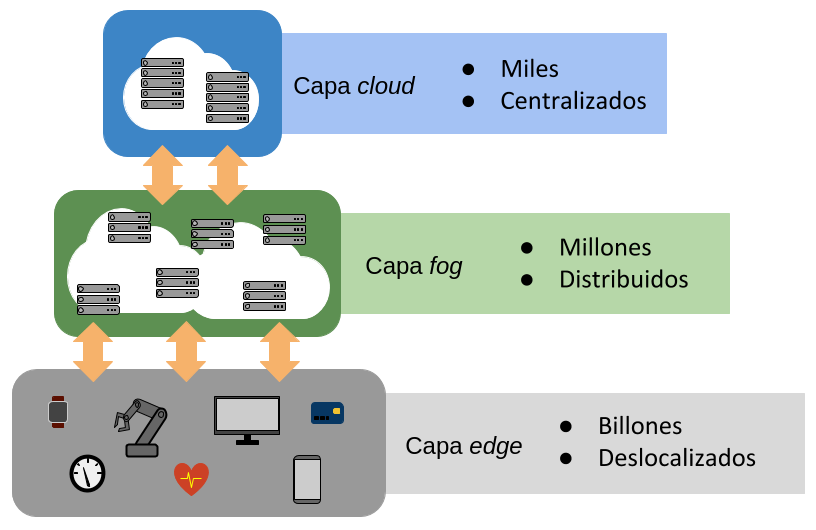
\includegraphics[width=0.7\textwidth]{02-state_of_the_art/cloud-fog-edge.png}
  \caption{Estructura por capas \textit{cloud-fog-edge}}
  \label{fig:02-cloud_fog_edge}
\end{figure}

Dejando atrás la ya explicada nube, vamos a adentrarnos más en el \textit{fog}.
Esta capa se compone de los llamados nodos \textit{fog}, que son los encargados
de llevar a cabo las distintas tareas. Cualquier dispositivo con capacidad de
procesamiento, memoria y conexión de red puede ser un nodo viable. De esta
forma, se pueden usar como nodos routers, switches y otros dispositivos de
redes, así como cámaras de videovigilancia. Se aprovecha la capacidad de
procesamiento de todos estos dispositivos cuando no se están usando al 100\%.
Como ya se ha indicado, estos nodos se encuentran ubicados en la misma red local
(LAN) que los dispositivos del borde de la red que generan los datos. Las
distintas tareas de análisis y control a realizar sobre estos datos se
distribuyen sobre los nodos \textit{fog} de forma dinámica dependiendo de la
carga de trabajo que posean los mismos. A la hora de asignar una tarea a un
nodo, siempre se debe intentar hacer de forma que el nodo elegido esté lo más
cerca posible de la fuente de los datos \cite{gedeon_fog_2018}. Esto es
especialmente importante para tareas de control, donde es posible que no todos
los nodos \textit{fog} de la planta tengan la latencia necesaria para cumplir
con los requisitos temporales. En este sentido, en \cite{pop_enabling_2018} se
propone el uso de TSN (\textit{Time-Sensitive Networking}) para las
comunicaciones en la capa \textit{fog}, con el objetivo de reducir estas
latencias. Este modelo de computación distribuida sobre una bolsa o
\textit{pool} de recursos es muy similar al que encontramos en la nube, con la
diferencia de que en el \textit{fog} estos recursos son mucho más limitados, por
lo que es también esencial optimizar el uso de los mismos. Debido a esta
similitud con el modelo de la nube, las mismas tecnologías de virtualización
usadas en ésta también son útiles en el nuevo paradigma \cite{yi_fog_2015}.
Algunos modelos ya han sido propuestos para la aplicación del \textit{fog} a los
sistemas industriales y el modelado de la Industria 4.0
\cite{verba_modeling_2019} \cite{tseng_lightweight_2018}.

Aunque la capacidad de procesamiento del \textit{fog} es mucho menor que la de
la nube, sigue siendo útil para realizar algunas tareas menos intensivas
evitando tener que desplazar todos los datos a la nube, con la latencia y la
carga en la red que eso supone. Como consecuencia del avance del IoT
(\textit{Internet of Things}) industrial, que es considerada una de las
tecnologías más importantes para la Industria 4.0 \cite{lu_industry_2017}, el
número de dispositivos presentes en las plantas y, por tanto, la cantidad de
datos que se generan va a ser mucho mayor, poniendo aún más presión sobre la
red, que es donde se podría producir el cuello de botella \cite{shi_edge_2016}.
El \textit{edge} trata de solucionar esto al reducir la cantidad de datos que se
deben enviar hacia las capas superiores procesando una parte de ellos de forma
local. Cabe destacar que el \textit{fog} también permite relajar el tráfico de
red \cite{wang_traffic_2019}. Los dispositivos del borde de la red, aún
ofreciendo menos potencia que la combinada del \textit{fog}, también pueden ser
usados para realizar algunas acciones sobre los datos. En concreto, las tareas
de control que requieran de un tiempo de respuesta más rápido pueden realizarse
en esta capa, tomando decisiones directamente sobre los datos que recoge el
dispositivo. Por otra parte, Khan \cite{khan_edge_2019} identifica la falta de
confianza en los sistemas \textit{edge} como uno de los principales problemas a
los que se enfrenta el paradigma, además de la integración de sistemas y la
movilidad. Esta falta de confianza es especialmente grave si pretendemos
desplegar sistemas de control críticos sobre plataformas de este tipo. Como
solución al problema de la confianza, Stanciu \cite{stanciu_blockchain_2017}
propone usar tecnología de \textit{blockchain} para desplegar sistemas de
control distribuidos en el \textit{edge}.

Sectores como el automovilístico, energético o de alimentación están muy
interesados en el desarrollo de la Industria 4.0 debido a los importantes
beneficios que se estima que puede tener para sus procesos. Gracias al 5G y a
las mejoras en las comunicaciones, el IoT se convierte en una idea capaz de dar
a las organizaciones una cantidad de información sobre sus procesos industriales
jamás vista antes. Estos datos son la base de la Industria 4.0
\cite{khan_perspective_2016}, ya que permiten la definición de sistemas
ciber-físicos y gemelos digitales que replican perfectamente los procesos
físicos en el plano digital, lo que abre la puerta a un control inédito sobre
dichos procesos. Además de las comunicaciones, otro reto muy importante para la
consecución de estos objetivos es el modelado de estos sistemas cuidando los
aspectos deseados de seguridad y fiabilidad \cite{farsi_industry_2019}. En este
sentido, creemos que el \textit{fog} es un modelo de computación que puede
facilitar el diseño de estos CPS al proporcionar una plataforma robusta y
unificada sobre la que implementarlos.

\section{Tecnologías de virtualización: hipervisores y contenedores}

\section{Aspectos de computación en tiempo real: RTOS, algoritmos de
  planificación y herramientas}
\label{sec:real-time}
